\documentclass{news}

\lang     {english}
\title    {The Ai Times:}
\subtitle {News, rumors, revelations, and prophecies from the age of artificial intelligence.}
\authors  {Alshival}
\keywords {newspaper, stories, journalism}
\date     {\today}
\location {Universal}
\cost     {}
\issue    {1}
\volume   {4}

\begin{document}

\by{Samuel Cavazos}{Top 100 Data \& Analytics Professional}{media/ait.png}

\hh{OpenAi Releasing a Macro Pad for Codex}

{\l{O}penAi is giving codex buttons. \href{https://www.theverge.com/ai-artificial-intelligence/959174/openai-codex-hardware-work-louder}{The Verge reports} that OpenAi is teasing a Codex-related hardware device in partnership with Work Louder, with a launch planned for July 15, 2026.
\par}

\begin{center}
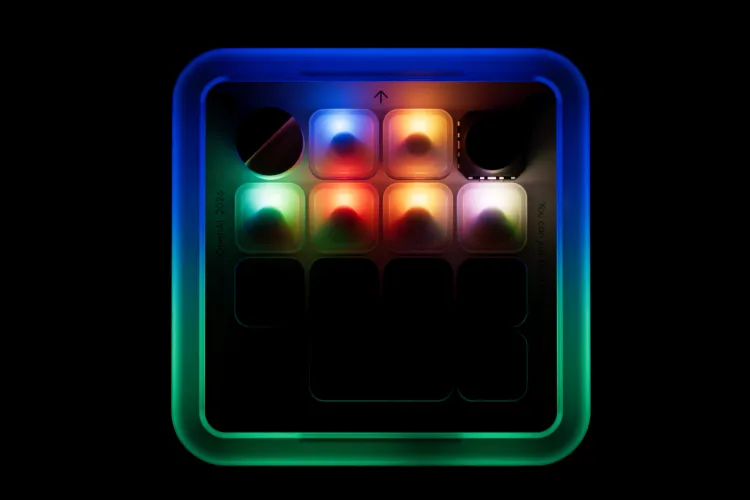
\includegraphics[width=\linewidth]{media/openai-work-louder.png}
\end{center}

This is not the top-secret \& highly anticipated Jony Ive device, which is still somewhere in the dream machine. Work Louder already makes mechanical keyboards and macro pads with programmable keys, dials, and switches. The device in OpenAi's teaser looks similar to Work Louder's Creator Micro 2, a small controller with 13 mechanical switches, a joystick, and a touch sensor. 

Codex is not just a chatbot anymore. It is becoming a workflow. Start task. Review diff. Run tests. Explain failure. Apply patch. Push branch. A physical button for ``summon the agent'' sounds silly until you realize programmers already buy keyboards with knobs because changing volume with a mouse is beneath us.

OpenAi is treating agentic coding like an environment with muscle memory. Figma did something similar with Work Louder for design shortcuts. OpenAi appears to be trying the same thing for software work: take the invisible AI assistant and give it a place on the desk. We are all for it. 

We do not know the price, exact layout, or whether this will be a Codex-branded macro pad or a limited collaboration. But we do know that we will do whatever we can to get our hands and test this device out for readers of \emph{The Ai Times}.

\hh{Robots Watch One Video, Then Wing It}
{Training robots requires doing the same task over and over again. Lots of time and resources goes into collecting training data for each task in a variety of different environments. But what if we could show the machine a single video and that was enough for it to learn? That is what ORION aims to do. 
\par}

\href{https://link.springer.com/article/10.1007/s10514-026-10253-8}{A new paper in \textit{Autonomous Robots}} pushes directly at that problem. The system is called ORION, short for Open-world video Imitation. The authors teach robot manipulation from a single RGB or RGB-D human demonstration video by extracting what they call Open-world Object Graphs.

The idea is useful. Instead of trying to copy the human's exact arm motion, ORION watches the objects. It builds a sequence of graph states: which task-relevant objects exist, where they are, how they relate to each other, when contact changes, and where a hand or gripper should interact. The graph becomes the plan.

The important claim is generalization. \href{https://ut-austin-rpl.github.io/ORION-release/}{The ORION project page} says the system learns from videos captured by ordinary devices and generalizes to new visual backgrounds, camera angles, spatial layouts, and novel object instances from the same categories. The Springer paper reports an average real-world success rate of 74.4\% across short-horizon and long-horizon tasks using RGB-D and RGB-only demonstrations.

There are limits. The paper focuses on tabletop manipulation with relatively clean object interactions, and the authors note that richer contact dynamics and force regulation remain future work. But this is still an important milestone in deep-learning for robotics.

Pixels are noisy. Human motion is messy. But a mug on a coaster, a chip on a plate, or juice being poured into a cup has structure. A graph structure. 

Thanks to the mathematicians who taught me graph theory during my studies, the paper was quite approachable and definitely worth reading.
\hh{One week. Two Tesla Crashes. }
{A 79-year-old woman from Agoura Hills was killed Monday, June 29, 2026, after a Tesla left the travel lane of a Simi Valley shopping-center parking lot and struck her outside an Urbane Cafe. \href{https://abc7.com/post/simi-valley-crash-1-killed-5-injured-car-slams-urbane-cafe-restaurant/19416545/}{ABC7 reports} that the Tesla jumped a curb, narrowly missed two customers, and crashed into the outdoor seating area of the restaurant.
\par}

\href{https://www.cbsnews.com/losangeles/news/simi-valley-target-parking-lot-urbane-cafe-deadly-crash-tierra-rejada-road/}{CBS Los Angeles reports} that Simi Valley police said the woman was walking on the sidewalk when she was struck by a vehicle that had left the parking lot's travel lane. She was pronounced dead at the scene. Five other people were injured, including the driver, a Thousand Oaks man, and three juvenile passengers. Police said there was no evidence at the time to indicate drugs or alcohol played a role.

The important line is the one we do not yet have. \href{https://abcnews.go.com/US/tesla-crashes-cafe-simi-valley-killing-1-injuring/story?id=134327301}{ABC News reports} that authorities have not said whether any driver-assistance technology was engaged.

A Tesla left the intended path in a low-speed pedestrian environment and killed a woman on a sidewalk. Was it FSD? It is unfortunate that we have to ask ourselves that question, but the pattern of freak accidents involving Tesla vehicles is impossible to ignore.

In \emph{The Ai Times} \href{https://github.com/Alshival-Ai/the-ai-times/blob/main/Vol%201/1.1/main.pdf}{Vol. 1 No. 1}, we wrote about a fatal Katy, Texas crash in which a Tesla reportedly failed to turn and drove into a home. In \href{https://github.com/Alshival-Ai/the-ai-times/blob/main/Vol%201/1.2/main.pdf}{Vol. 1 No. 2}, we followed the lawsuit and the unresolved questions around which version of Tesla's automated-driving feature was active. We will keep you updated on these stories as new information becomes available.

\hh{Announcements}

\textit{The Ai Times} is now on Substack. Scan the code below to get each new issue, along with the sources, side quests, and stray prophecies that did not fit on the page.

\begin{minipage}[c]{.50\linewidth}
{\large\cinzel
{\normalsize The }

\qquad Ai

\qquad\quad Times}
\end{minipage}%
\begin{minipage}[c]{0.50\linewidth}

\includegraphics[width=\linewidth]{media/ai-times-qr.png}
\end{minipage}

\end{document}
